\section{Background}
Many of todays smart phones are running Android as their operating system, and  data claims it dominates the market with an 87.6\% share in the second quarter of 2016\cite{idc}. Making it essenstial for future mobile forensic work, for gathering information in an investigation.

When an investigation occurs, there are several approaches to data acquisistion: (1) Manual acquisition, (2) Logical acquisition, (3) Physical acquisition, (4) Brute force acquisition. The field of interest for this paper is physical acquisition of the primary storage; it focuses primarly on creating a bit-by-bit copy of the random access memory (RAM). Due to RAM being volatile, it is often the target of stealthy illegal activites to avoid leaving data. If data was stored in the flash drive, it would still be resident until OS tries to overwrite the same physical area and garbage collector is initiated. The point being that data residing on a secondary storage device, will be living longer and probably be logged more extensively.

The Android OS is in short words a Linux-based OS, where most OS tasks are performed by open source C libraries, and Java is used for the development of Android applications. These applications are compiled to bytecode for the Java virtual machine (JVM), which is then translated for a second virtual machine which executes them. Depending on which version of Android a smart phone is running, different virtual machines are used for execution.
For Android versions 4.4 and prior, Dalvik was used. It was replaced by ART in 4.5, and is still the de-facto standard.

Why does this matter? The virtual machines that are used are suppose to run Java applications, and have therefore gained several features of the Java programming language. One of these features are the memory management module, which has a built-in garbage collector(GC). It lets the user create objects without worrying about memory allocation and deallocation. Reducing the need for boilerplate code, and problems with memory leaks and such, which often are languages like C and C++ are subject to. 

The GC have the job of cleaning RAM, therefore removing potential information to be gathered. It is therefore of severe importance, that data residing in memory gets gathered before the device eventually power offs, or the garbage collector initializes.

Both ART and Dalvik use by default a method called "concurrent mark and sweep" for their GC\cite{ARTGC,DALVIKGC}. It works by traversing the heap for objects that are "reachable" or used by applications, those who are not will be regarded as free space again. Making space for potential new data to be stored within it. A figure of the process, can be seen at figure \ref{fig:mas}. Generally the heap is a region of the memory that is regarded as free memory for any process to use, however in Java it is used to store all objects created. Therefore the GC may potentially remove one of the better sources for information, the objects. The good news are that once data is freed, no overwriting is enforced; in other words, data is not overwritten until another object takes its place\cite{DALVIKGC}; in addition to each application running its own garbage collector and private heap, making the RAM data resident for possibly long periods of time\cite{AndroidMemManagement}.

\begin{figure}[h]
  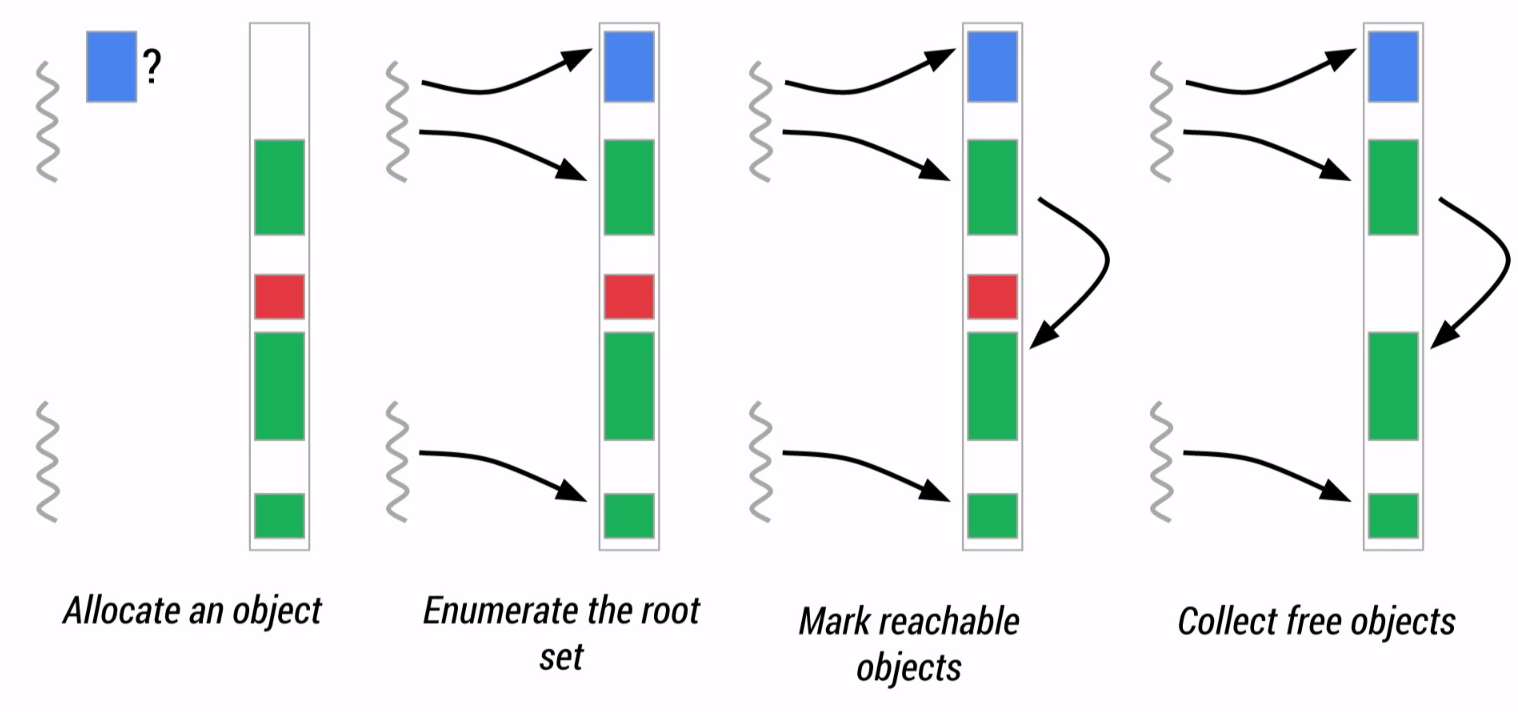
\includegraphics[width=0.5 \textwidth]{gc}
  \caption{Mark and Sweep\cite{ARTGC}}
  \label{fig:mas}
\end{figure}

Because all objects created in the heap, there may be a potential trace of information of an application. Through the use of several popular online communication applications, the amount of data that can be collected through a memory dump will be explored; despite knowing that the GC might start, or extra security measures might prevent us to do so.

\subsection{Forensics Process}
A digital forensics process is used in order to conduct the most thorough analysis of the data of a device, and prevent investigators from making mistakes. It also helps ensuring that every step of the process is documented. \r{A}rnes et al. describes a process with five stages: Identification, collection, examination, analysis and presentation\cite{DiFoBook}. The process in itself is an iterative process, and specifically the phases of collection, examination and analysis are done over and over again in some cases. The digital forensics process presented here is a generic process, which means it can be used on every digitial device there is. By using a digital forensics process like this, the investigators are able to keep the integrity of the data and also document chain of custody which is important when a case is going to court. \\

Preparation is important in the phase of identification. When looking for a mobile device, it is essential to bring equipment to charge the device in case it is turned on (live), because there may be data on the device that will disappear if is turned off, for instance data in the RAM. Devices that are turned off (dead) should not be turned on, because it can destroy data. Mobile devices that are live at the crime scene should be put in a box that isolates it from networks and blocks signals. The box will prevent the mobile device from for example remote deletion or tampering of the data on it\cite{DiFoBook}. 

The collection phase consists of retrieving data from the device (or devices) that are brought in by the investigators\cite{DiFoBook}. Brezinski and Killalea\cite{RFC3227} suggests evidence collection to be done in an order of volatility. In the case of a mobile device, the RAM should therefore be collected before the primary storage. This is done by copying data over to another system from the mobile device. While a regular copy may cause the system to overwrite existing data, write-blockers are used in order to deny the system anything other than read access, which makes a copy doable without interfering with the existing content on the device. A hash of both the copied device and the copy itself is then created, and compared so that it is no doubt that the content of the copy matches the original device\cite{DiFoBook}.This is done in order to keep the integrity of the actual system, while investigators can work on the copy of it. 

Examination is the process of finding data aqcuired in the collection phase which might be of interest to the specific case. Forensics tools can for instance be used to categorize the data found on the mobile device, and at the same time track what the investigator is doing. Some tools also offers the capability of automatically removing known files used by the operating system, which makes the process of filtering out gigabytes of date easier for the investigator of the device.

After the phase of examination is done, analysis is done in order to see if the files contain information that might be useful in the case. This may be everything from photos, text messages or GPS localization data of the device. Timelines are often used as a help to determine what happened in what order. Log files or meta data like time stamps from files can help create a timeline, which gives a better overview of what has happened. The timeline created can then be expanded to contain real-life activities, which helps the investigator further understand the data. Note that when this process is done, i.e. one device has gone through the collection phase, examination phase and analysis phase, the same process starts again for a new device that might be relevant to the case. After all the devices has gone through these stages of the process, the presentation phase is started.
